
\section{Theorie}
\label{sec:Theorie}

\subsection{Die allgemeinen Eigenschaften einer LC-Kette}
Eine LC-Kette ist eine Verkettung von n in Reihe geschalteten LC-Gliedern.
 Jedes dieser Glieder hat die Eigenschaften eines Tiefpasses und lässt
  Wechselspannungen mit geringen Frequenzen passieren, während es hochfrequente jedoch
   blockiert. Verfeinert man die Anzahl der Kettenglieder und lässt
   deren Anzahl $\to \infty$ laufen, erhält man eine unendliche LC-Kette. Letztere
    beschreibt ein Ersatzschaltbild einer elektrischen Leitung, im Fall der
     LC-Kette einer verlustfreien Leitung. Es zeigt sich, dass eine unendliche
      Kette einen spezifischen Gesamtwiderstand, den Wellenwiderstand $Z$, besitzt.
      Dieser ist rein reell und nur von der Generatorfrequenz abhängig. Für ihn gilt:
      \begin{equation}
        Z(f) = \sqrt{\frac{L}{C}} \cdot \frac{1}{2\pi \sqrt{1-0,25\omega² LC}}
      \end{equation}

 Zum anderen kann die LC-Kette auch als System gekoppelter
    Schwingungen betrachtet werden, welches eine Vielzahl von Eigenschwingungen besitzt.
      Aufgrunddessen können Wellen und Wellenpakete auf ihr übertragen werden.
	Eine Welle besitzt eine Phasengeschwindigkeit, mit der sie sich im Medium ausbreitet. Für sie gilt
\begin{equation}
v_{ph} = \frac{\omega}{\theta}\text{.}
\end{equation} 
	$\theta$ beschreibt dabei den Phasenunterschied pro Kettenglied. Auf ihn wird später näher eingegangen.
     Da ein Wellenpaket aus einer Menge unterschiedlicher Einzelwellen besteht
      und jede eine eigene Phasengeschwindigkeit besitzt, kommt es zu einer Verzerrung
  der Gestalt des Wellenpaketes. Diesen Effekt nennt man Dispersion.


     \begin{figure}[H]
       \centering
       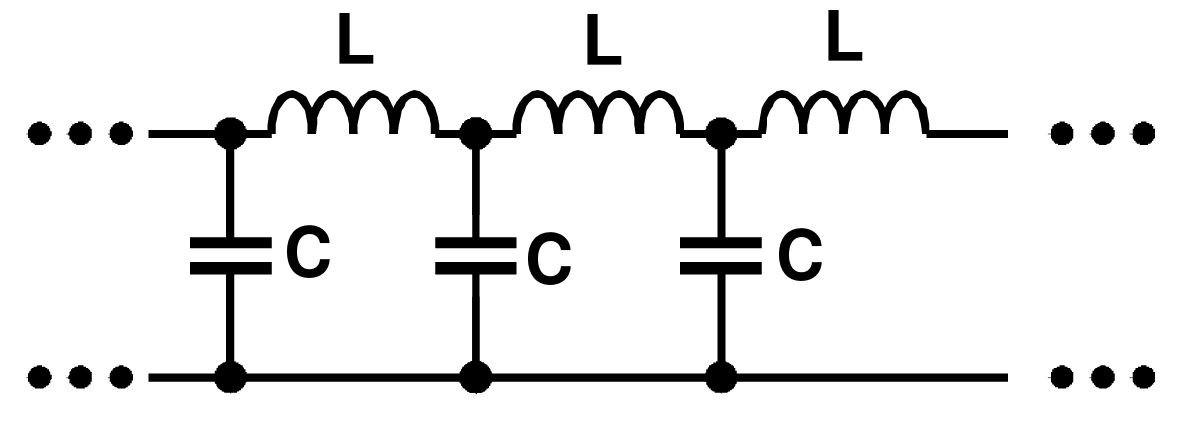
\includegraphics[width=\linewidth-200pt,height=\textheight-200pt,keepaspectratio]{content/Grafiken/LCKette.png}
       \caption{Die unendliche LC-Kette}
       \label{fig:LC-Kette}
     \end{figure}

\subsection{Die Eigenschaften einer unendlichen LC-Kette}


Im folgenden wird weiter auf die bereits gennanten Effekte eingegangen. Zunächst
 wird die einfache $LC$-Kette thematisiert. Diese besitzt nur Kondensatoren der
 gleichen Kapazität $C$.\\\\

Aus den kirchhoffschen Regeln folgt die BewegungsDGL:
\begin{equation}
- \omega ^2 C U_n + \frac{1}{L} \left( -U_{n-1} + 2U_ n -U{n-1} \right) = 0
\end{equation}

Mit einem komplexen E-Ansatz gelangt man zu:
\begin{equation}
 f ^2 = \frac{1}{2LC\pi^2}(1-cos\theta)
\end{equation}
Dieser Ausruck wird als Dispersionsrelation beschrieben und stellt die Änderung
 der Phase pro Kettenglied in Abhängigkeit der Frequenz dar. Anhand der Formel lässt sich erkennen,
  dass der Frequenzbereich indem Schwingungen auftreten begrenzt ist. Daher bilden sich
   für Frequenzen $\geq \frac{1}{\sqrt{LC\pi^2}}$ keine Schwingungen aus.\\\\

 Nun wird die $LC_1C_2$-Kette näher betracht. Sie besitzt Kondensatoren mit zwei
  verschiedenen Kapazitäten $C_1$ und $C_2$, welche im Wechsel verbaut sind.
 Aus den kirchhoffschen Regeln folgen die BewegungsDGLn:
 \begin{equation}
   -\omega^2 C_1 U_{2n+1} + \frac{1}{L} \left( -U_{2n} + 2U_{2n+1} - U_{2n+2} \right) = 0
 \end{equation}
 und
 \begin{equation}
   -\omega^2 C_2 U_{2n} + \frac{1}{L} \left( -U_{2n-1} + 2U_{2n+1} - U_{2n+1} \right) = 0
 \end{equation}

Es folgt für die auftretende Dispersion:
\begin{equation}
  f_{1/2}^2 = \frac{1}{4\pi^2L}\left(\frac{1}{C_1}+\frac{1}{C_2}\right) \pm \frac{1}{4\pi^2L}\sqrt{\left(\frac{1}{C_1}+\frac{1}{C_2} \right)^2 - \frac{4 sin^2\theta}{C_1C_2}}
\end{equation}
Es zeigt sich, dass die $LC_1C_2$-Kette aufgrund der positiven und negativen Wurzel
zwei Frequenzbereiche besitzt in denen Schwingungen auftreten. Die Verläufe der Unteren und Oberen
 Grenzfrequenz werden akustischer bzw. optischer Ast genannt. Wird mit
$sin \theta \approx \theta$ genähert, erhält man einen Kurvenverlauf, welcher ca. so aussieht:

 \begin{figure}[H]
   \centering
   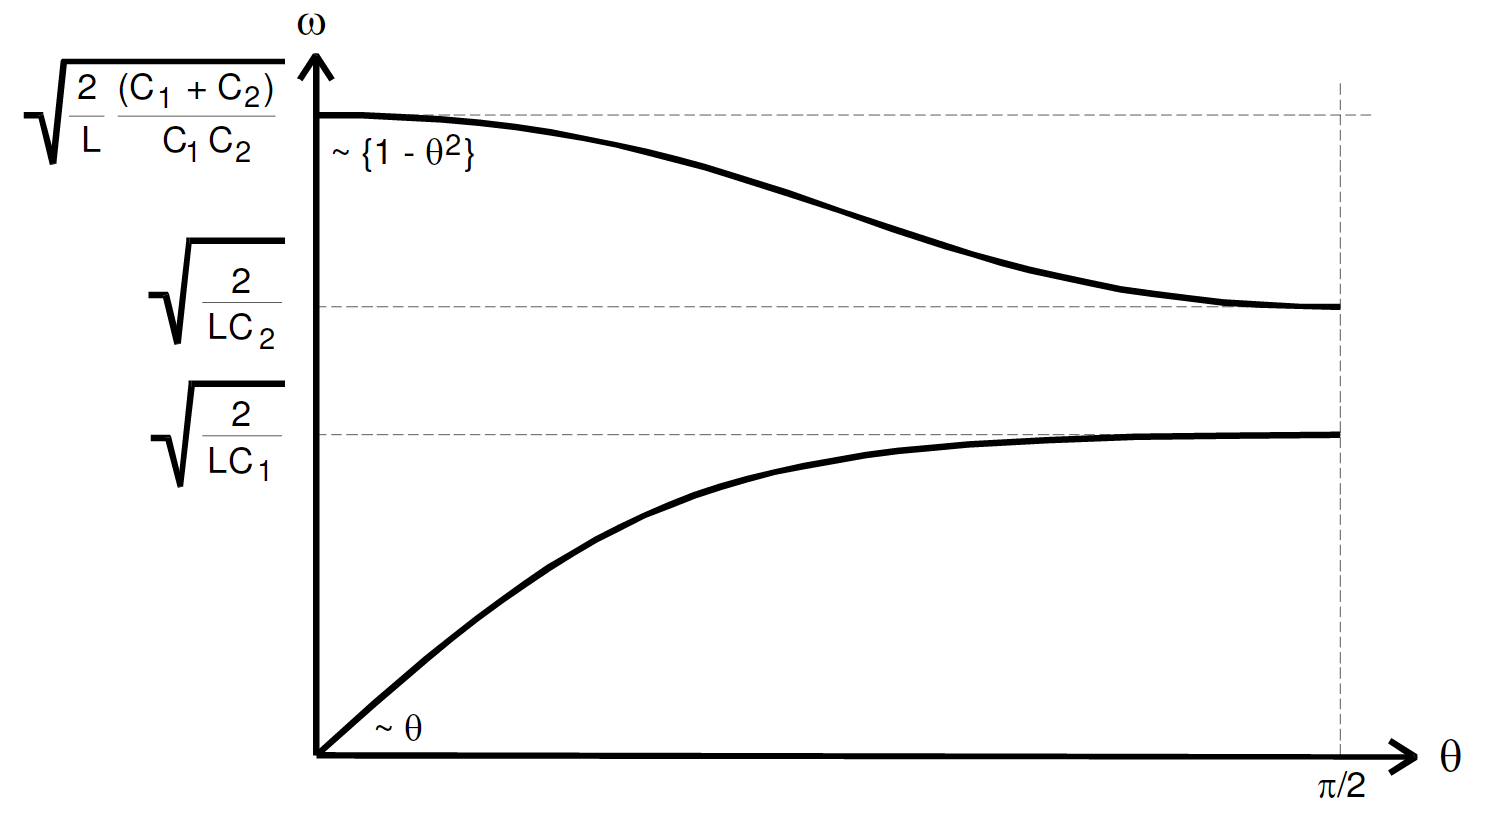
\includegraphics[width=\linewidth-200pt,height=\textheight-200pt,keepaspectratio]{content/Grafiken/Dispersionskurven.png}
   \caption{Die nötige Frequenz in Abhängigkeit der Dispersion}
   \label{fig:LC-Kette}
 \end{figure}


\subsection{Die Eigenschaften einer endlichen LC-Kette}
Liegt eine LC-Kette endlicher Länge vor, bzw. wurden Anfangs und Endwiderstand
 nicht nach Formel () der Frequenz des Wechselsstromes ensprechend angepasst,
  kommt es zur Reflexion ankommender Wellen. Aus den kirchhoffschen Regeln folgt das Verhältnis:
  \begin{equation}
    \frac{U_{ref}}{U_{ein}} = \frac{R-Z}{R+Z}\text{.}
  \end{equation}
  Es folgen die Spezialfälle:\\

  a) Die LC-Kette besitzt ein offens Ende, $R$ beträgt also $\infty$. An diesem
   wird eine ankommende Welle vollständig und ohne Phasensprung reflektiert.\\

  b) Die LC-Kette ist kurzgeschlossen, $R$ beträgt daher 0. An diesem Ende wird
   eine ankommende Welle vollständig reflektiert, jedoch mit einem Phasensprung von $\pi$.\\

 c) Werden Anfangs und Endwiderstand auf den Wellenwiderstand der LC-Kette eingestellt,
  so verhält sie sich wie eine unendliche LC-Kette. Aus diesem Grund kommt es auch nicht zur Reflexion.
